
\documentclass[12pt]{mitthesis}
\usepackage{titlesec}
\usepackage{geometry}
\usepackage{graphicx}
\usepackage{booktabs, chemformula}
\usepackage{titlesec, blindtext, color}
\usepackage{listings}
\usepackage{natbib}
\usepackage{xcolor} 
\pagestyle{plain}

\begin{document}

\tableofcontents

\pagestyle{plain}

\chapter{Presentation of the research topic}

The domain of the proposed thesis is Automated Software Engineering. The thesis will develop methods for the analysis of legacy software systems, focusing on using historical information describing the evolution of the systems extracted from the versioning systems. 
The methods for analysis will integrate techniques based on computational algorithms as well as data-mining. As proof-of-concept, tool prototypes will implement the proposed methods and validate them by extensive experimentation on several cases of real-life systems.

\chapter{Software evolution and maintainability}
\section{Software evolution}
Software evolves 

P. Brooks \cite{Brooks:1987:NSB:26440.26441} notes the following properties of large software systems:

\begin{figure}[H]
\centering
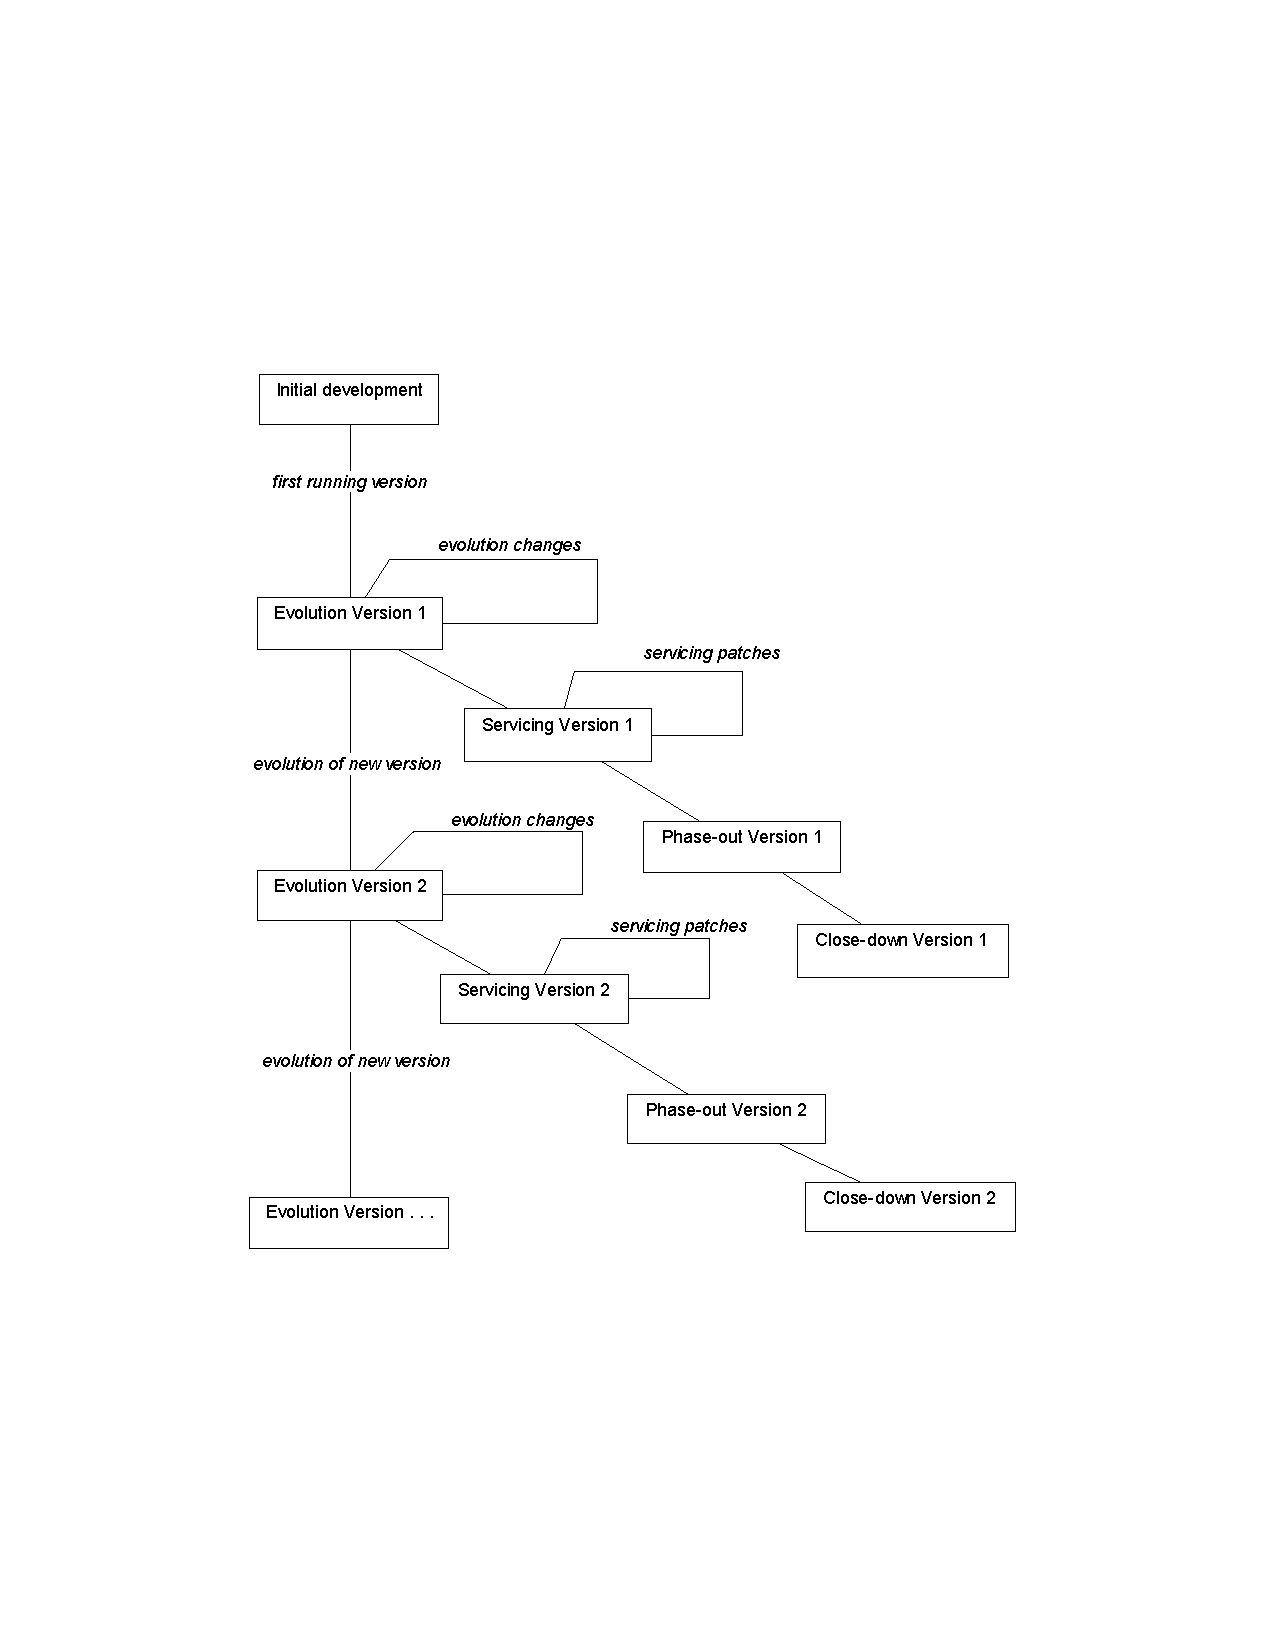
\includegraphics[width=\textwidth]{staged_model.pdf}
\label{fig:The versioned staged model}
\end{figure}

\section{Software maintenance}
In early days software maintenance was a small part of the software life cycle. As time was passing and more software was created, people realized that software does not die. Even if the actual development of the software may be frozen, requests regarding bug fixing and compatibility with new operating systems may appear over time. Sometimes software maintenance requires more effort than to build the system from scratch \cite{Yang:2003:SES:599790}.

Lientz and Swanson categorised maintenance activities into four classes \cite{Lientz:1981:PAS:358790.358796}:
\begin{itemize}
\item Adaptive maintenance: changes in the software environment.
\item Perfective maintenance: new user requirements and documentation improvement.
\item Corrective maintenance: debugging anf bug fixing.
\item Preventive maintenance: prevent future problems.
\end{itemize}

They also made a survey on the problems of application software maintenance in 487 organizations. The survey showed that most of the maintenance effort was on the first two types (adaptive and perfective maintenance). Many other studies suggest similar results.\cite{Bennett}
All these studies underline one thing: \textit{the incorporation of new user requirements is the main problem for software evolution and maintenance} \cite{Lientz:1981:PAS:358790.358796}.

One may ask why maintenance requires so much effort? There are some main problem factors when it comes to maintenance:

\begin{itemize}
\item User knowledge: lack of user training and/or lack of understanding of the system.
\item Programmer effectiveness: lack of skills or experience for maintenance, development.
\item Product quality: quality of the original system, quality of documentation and specs.
\item Machine requirements: increasing storage or decreasing processing time requirements.
\item System reliability: data integrity, hardware, and software reliability.
\end{itemize}

\section{Software quality}

\chapter{Dependencies in software systems}
A dependency is created by two elements that are in a relationship and indicates that an element of the relationship, in some manner, depends on the other element of the relationship \cite{Booch:2004:OAD:975416}, \cite{Cataldo2009SoftwareDW}.

A developer gains information about a software system by looking at it in two different ways: 
\begin{itemize}
	\item top-down: starting from the highest level of abstraction of the system and going down to the code.
	\item bottom-up: starting from the code and going up to the highest level of abstraction.
\end{itemize}

Both ways imply gradually gaining new information about the system and in both, the developer traces the dependencies and connections of the software system \cite{Wilde90understandingprogram}, \cite{341244}.

\section{Structural dependencies}
Structural dependencies can be found by analysing the source code. \cite{Sangal:2005:UDM:1094811.1094824}. 
There are several types of relationships between these source code entities and all those create \textit{structural dependencies}:

\subsubsection{Data Item Dependencies}
Data items can be variables, records or structures. A dependency is created between two data items when the value held in the first data item is used or affects the value from the second.

\subsubsection{Data Type Dependencies}
Data items are declared to be of a specific data type. Besides the built-in data types that every programming language has, developers can also create new types that they can use. Each time the data type definition is changed it will affect all the data items that are declared to be of that type. 

\subsubsection{Subprogram Dependencies}
A subprogram is a sequence of instructions that performs a certain task. Depending on the programming language a subprogram may also be called a routine, a method, a function or a procedure. When a subprogram is changed, the developer must check the effects of that change in all the places that are calling that subprogram. Subprograms may also have dependencies with the data items that they receive as input or the data items that they are computing.


\section{Logical dependencies}
\subsection{Co-change filtering}


\chapter{Usage of dependencies}

\section{Fault detection}
past changes are good predictors of future faults
\section{Architectural reconstruction}
Currently, the software systems contain tens of thousands of lines of code and are updated multiple times a day by multiple developers.  In order to successfully accomplish a task as a developer in such a system, you need to have a clear overview of the entire system and its connections. If for small systems a short look through the code can give the developer a good overview of the data-flow and functionalities of the system, in systems with tens of thousands of lines of code that's impossible. That is one of the reasons why the system's architecture is needed.
\section{Software metrics}

\chapter{Problems in Dependency Tracing}

%%%%%%%%%%%%%%%%%%%%%%%%%%%%%%%%%%%%%%%%%%%%%%%%%%%%%%%%%%%%%%%%%%%%%%%%%%%%%%%%

\chapter{Current status of research}

The current trend recommends that general dependency management methods and tools should also include logical dependencies besides the structural dependencies \cite{Oliva:2011:ISL:2067853.2068086}, \cite{DBLP:journals/jss/AjienkaC17}. 

Software engineering practice has shown that sometimes modules which do not present structural dependencies still appear to be related. Co-evolution represents the phenomenon when one component changes in response to a change in another component \cite{Yu:2007:UCC:1231330.1231370}. Those changes can be found in the software history maintained by the versioning system. Gall \cite{Gall:1998:DLC:850947.853338} identified as logical coupling between two modules the fact that these modules  \textit{repeatedly} change together during the historical evolution of the software system. 
 \textit{Logical dependencies} (a.k.a logical coupling) can be found by software history analysis and can reveal relationships that are not always present in the source code (structural dependencies).  

The concepts of logical coupling and logical dependencies were first used in different analysis tasks, all related to changes: for software change impact analysis \cite{1553643}, for identifying the potential ripple effects caused by software changes during software maintenance and evolution \cite{DBLP:conf/issre/OlivaG15}, \cite{Oliva:2011:ISL:2067853.2068086}, \cite{Poshyvanyk2009}, \cite{posh2010} or for their link to deffects \cite{wiese}, \cite{Zimmermann:2004:MVH:998675.999460}.

Different applications based on dependency analysis could be improved if, beyond structural dependencies, they also take into account the hidden non-structural dependencies. For example, works  which investigate different methods for architectural reconstruction \cite{SoraConti}, \cite{SoraSem13}, \cite{PagerankENASE},  all of them based on the information provided by structural dependencies, could enrich their dependency models by taking into account also logical dependencies. However, a thorough survey \cite{sar} shows that historical information has been rarely used in architectural reconstruction. 

Another survey \cite{Shtern:2012:CMS:2332427.2332428} mentions one possible explanation why historical information have been rarely used in architectural reconstruction: the size of the extracted information. One problem is the size of the extraction process, which has to analyze many versions from the historical evolution of the system. Another problem is the big number of pairs of classes which record co-changes and how they relate to the number of pairs of classes with structural dependencies.

%%%%%%%%%%%%%%%%%%%%%%%%%%%%%%%%%%%%%%%%%%%%%%%%%%%%%%%%%%%%%%%%%%%%%%%%%%%%%%%%
\chapter{Co-changes filtering}
The software architecture is important in order to understand and maintain a system. Often code updates are made without checking or updating the architecture. This kind of updates cause the architecture to drift from the reality of the code over time.\cite{sar}
So reconstructing the architecture and verifying if still matches the reality is important. 

Surveys show that architectural reconstruction is mainly made based on structural dependencies \cite{Shtern:2012:CMS:2332427.2332428} \cite{sar}, the main reason why historical information is rarely used in architectural reconstruction is the size of the extracted information.

Logical dependencies should integrate harmoniously with structural dependencies in an unitary dependency model: valid logical dependencies should not be omitted from the dependency model, but structural dependencies should not be engulfed by questionable logical dependencies generated by casual co-changes.  
Thus, in order to add logical dependencies besides structural dependencies in dependency models, class co-changes must be filtered until they remain only a reduced but relevant set of valid logical dependencies. 

Currently there is no set of rules or best practices that can be applied to the extracted class co-changes and can guarantee their filtering into a set of valid logical dependencies.
This is mainly because not all the updates made in the versioning system are code related. For example a commit that has as participants a big number of files can indicate that a merge with another branch or a folder renaming has been made. In this case, a series of irrelevant co-changing pairs of entities can be introduced. So, in order to exclude this kind of situations the information extracted from the versioning system has to be filtered first and then used.

Other works have tried to filter co-changes \cite{Oliva:2011:ISL:2067853.2068086}, \cite{DBLP:journals/jss/AjienkaC17}. One of the used co-changes filter is the commit size.The commit size is the number of code files changed in that particular commit. 
Ajienka and Capiluppi established a threshold of 10 for the maximum accepted size for a commit \cite{DBLP:journals/jss/AjienkaC17}. This means that all the commits that had more than 10 code files changed where discarded from the research. But setting a harcoded threshold for the commit size is debatable because in order to say that a commit is big or small you have to look first at the size of the system and at the trends from the versioning system. Even thought the best practices encourage small and often commits, the developers culture is the one that influences the most the trending size of commits from one system.

Filtering only after commit size is not enought, this type of filtering can indeed have an impact on the total number of extracted co-changes, but will only shrink the number of co-changes extracted without actually guaranteeing that the remaining ones have more relevancy and are more logical linked.

Although, some unrelated files can be updated by human error in small commits, for example: one file was forgot to be commited in the current commit and will be commited in the next one among some unrelated files. This kind of situation can introduce a set of co-changing pairs that are definetly not logical liked. In order to avoid this kind of situation a filter for the occurrence rate of co-changing pairs must be introduced. Co-changing pairs that occur multiple times are more prone to be logically dependent than the ones that occur only once. Currently there are no concrete examples of how the threshold for this type of filter can be calculated. In order to do that, incrementing the threshold by a certain step will be the start and then studying the impact on the remaining co-changing pairs for different systems. 

Taking into account also structural dependencies from all the revisions of the system was not made in previous works, this step is important in order to filter out the old, out-of-date logical dependencies. Some logical dependencies may have been also structural in previous revisions of the system but not in the current one. If we take into consideration also structural dependencies from previous revisions then the overlapping rate between logical and structural dependencies could probably increase. Another way to investigate this problem could be to study the trend of concurrences of co-changes: if co-changes between a pair of classes used to happen more often in the remote past than in the more recent past, it may be a sign that the problem causing the logical coupling has been removed in the mean time. 

Also, logical dependency can be also a structural dependency and vice-versa, so studying the overlapping between logical and structural dependencies while filtering is important since the intention is to introduce those logical dependencies among with structural dependencies in architectural reconstruction systems. Current studies have shown a relatively small percentage of overlapping between them with and without any kind of filtering \cite{DBLP:journals/jss/AjienkaC17}. This means that a lot of non related entities update together in the versioning system, the goal here is to establish the factors that determine such a small percentage of overlapping.


 %%%%%%%%%%%%%%%%%%%%%%%%%%%%%%%%%%%%%%%%%%%%%%%%%%%%%%%%%%%%%%%%%%%%%%%%%%%%%%%%

\chapter{Research content and stages of research}

\section{Proposed research stages}
The research will be made by following the next stages of implementation:


\textbf{A.} DEVELOPMENT OF CONTENT AND TOOLS

\textbf{Stage 1:} Build tool to extract structural dependencies from code and co-changes from git for a given set of projects.

\textbf{Stage 2:} Find filters for the co-changes extracted, the filters can be the ones already mentioned in previous works or new ones. Establish different thresholds for those filters.

\textbf{Stage 3:} Study the impact of those filters and the coresponding thresholds on the remaining quantity of co-changes for each system.
Study the overlappings between the remaining pairs of co-changing entites and the structural dependencies extracted. \cite{enase19}

\textbf{Stage 4:} Establish a dynamic way to determine the thresholds for filters in order to fit the best each studied sistem. Main focus on the threshold for number of occurences of co-changing pairs.
Use plots or other visual instruments in order to see the highests and the lowest rates for the numbers of occurrences among co-changing pairs.
Also filter those rates into normal and abnormal ones and study what was the cause of the highest rates (code or human related).

\textbf{Stage 5:} Take into account also structural dependencies from all the revisions of the system to filter out the old, out-of-date logical dependencies. 
Study how this affects the remaining number of logical dependencies.Here an extra check is needed, it can be a case in which old structural dependencies that were also logically linked to continue to be logically linked
even after the structural dependency was removed.

\textbf{B.} USAGE

\textbf{Stage 6:} Export the remaining co-changes whom at this step we can call logical dependencies and use them among structural dependencies in tools for architectural reconstruction to evaluate the improvement.

\textbf{Stage 7:} Compare the number of logical dependencies with metrics like Fan Out, Fan In, Efferent Coupling (Ce), Afferent Coupling (Ca) and study their connections.

\textbf{Stage 8:} Identify other tools that use historical information and evaluate the impact of co-changes filtering into logical dependences for them. 

\section{Gantt chart}

\begin{figure*}[h]
\centering
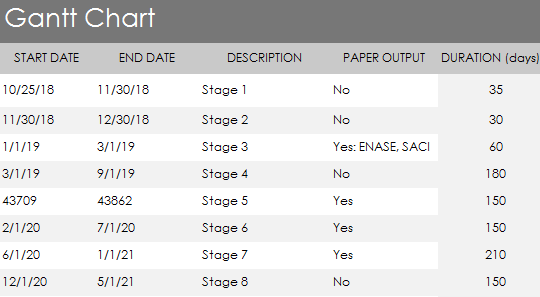
\includegraphics[width=\textwidth]{gantt_chart.PNG}
\label{fig:gantt1}
\end{figure*}

\begin{figure*}[h]
\centering
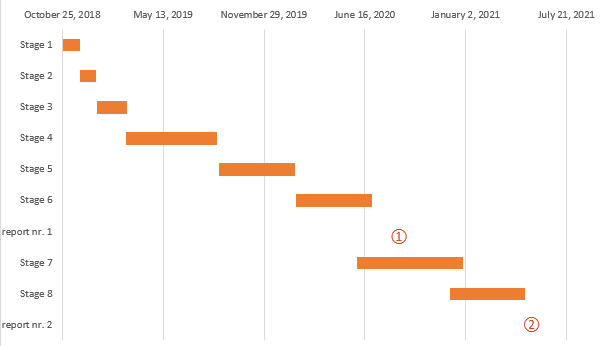
\includegraphics[width=\textwidth]{gantt_plot.PNG}
\label{fig:gantt2}
\end{figure*}

\section{Proposed contents of the thesis}

\bibliographystyle{plain}
\bibliography{logicaldepd}
\end{document}

